\documentclass[]{article}
\usepackage{lmodern}
\usepackage{amssymb,amsmath}
\usepackage{ifxetex,ifluatex}
\usepackage{fixltx2e} % provides \textsubscript
\ifnum 0\ifxetex 1\fi\ifluatex 1\fi=0 % if pdftex
  \usepackage[T1]{fontenc}
  \usepackage[utf8]{inputenc}
\else % if luatex or xelatex
  \ifxetex
    \usepackage{mathspec}
    \usepackage{xltxtra,xunicode}
  \else
    \usepackage{fontspec}
  \fi
  \defaultfontfeatures{Mapping=tex-text,Scale=MatchLowercase}
  \newcommand{\euro}{€}
\fi
% use upquote if available, for straight quotes in verbatim environments
\IfFileExists{upquote.sty}{\usepackage{upquote}}{}
% use microtype if available
\IfFileExists{microtype.sty}{%
\usepackage{microtype}
\UseMicrotypeSet[protrusion]{basicmath} % disable protrusion for tt fonts
}{}
\usepackage[margin=1in]{geometry}
\usepackage{color}
\usepackage{fancyvrb}
\newcommand{\VerbBar}{|}
\newcommand{\VERB}{\Verb[commandchars=\\\{\}]}
\DefineVerbatimEnvironment{Highlighting}{Verbatim}{commandchars=\\\{\}}
% Add ',fontsize=\small' for more characters per line
\usepackage{framed}
\definecolor{shadecolor}{RGB}{48,48,48}
\newenvironment{Shaded}{\begin{snugshade}}{\end{snugshade}}
\newcommand{\KeywordTok}[1]{\textcolor[rgb]{0.94,0.87,0.69}{{#1}}}
\newcommand{\DataTypeTok}[1]{\textcolor[rgb]{0.87,0.87,0.75}{{#1}}}
\newcommand{\DecValTok}[1]{\textcolor[rgb]{0.86,0.86,0.80}{{#1}}}
\newcommand{\BaseNTok}[1]{\textcolor[rgb]{0.86,0.64,0.64}{{#1}}}
\newcommand{\FloatTok}[1]{\textcolor[rgb]{0.75,0.75,0.82}{{#1}}}
\newcommand{\CharTok}[1]{\textcolor[rgb]{0.86,0.64,0.64}{{#1}}}
\newcommand{\StringTok}[1]{\textcolor[rgb]{0.80,0.58,0.58}{{#1}}}
\newcommand{\CommentTok}[1]{\textcolor[rgb]{0.50,0.62,0.50}{{#1}}}
\newcommand{\OtherTok}[1]{\textcolor[rgb]{0.94,0.94,0.56}{{#1}}}
\newcommand{\AlertTok}[1]{\textcolor[rgb]{1.00,0.81,0.69}{{#1}}}
\newcommand{\FunctionTok}[1]{\textcolor[rgb]{0.94,0.94,0.56}{{#1}}}
\newcommand{\RegionMarkerTok}[1]{\textcolor[rgb]{0.80,0.80,0.80}{{#1}}}
\newcommand{\ErrorTok}[1]{\textcolor[rgb]{0.76,0.75,0.62}{{#1}}}
\newcommand{\NormalTok}[1]{\textcolor[rgb]{0.80,0.80,0.80}{{#1}}}
\usepackage{graphicx}
\makeatletter
\def\maxwidth{\ifdim\Gin@nat@width>\linewidth\linewidth\else\Gin@nat@width\fi}
\def\maxheight{\ifdim\Gin@nat@height>\textheight\textheight\else\Gin@nat@height\fi}
\makeatother
% Scale images if necessary, so that they will not overflow the page
% margins by default, and it is still possible to overwrite the defaults
% using explicit options in \includegraphics[width, height, ...]{}
\setkeys{Gin}{width=\maxwidth,height=\maxheight,keepaspectratio}
\ifxetex
  \usepackage[setpagesize=false, % page size defined by xetex
              unicode=false, % unicode breaks when used with xetex
              xetex]{hyperref}
\else
  \usepackage[unicode=true]{hyperref}
\fi
\hypersetup{breaklinks=true,
            bookmarks=true,
            pdfauthor={Antoine Baldassari},
            pdftitle={Homework \#3},
            colorlinks=true,
            citecolor=blue,
            urlcolor=blue,
            linkcolor=magenta,
            pdfborder={0 0 0}}
\urlstyle{same}  % don't use monospace font for urls
\setlength{\parindent}{0pt}
\setlength{\parskip}{6pt plus 2pt minus 1pt}
\setlength{\emergencystretch}{3em}  % prevent overfull lines
\setcounter{secnumdepth}{0}

%%% Use protect on footnotes to avoid problems with footnotes in titles
\let\rmarkdownfootnote\footnote%
\def\footnote{\protect\rmarkdownfootnote}

%%% Change title format to be more compact
\usepackage{titling}

% Create subtitle command for use in maketitle
\newcommand{\subtitle}[1]{
  \posttitle{
    \begin{center}\large#1\end{center}
    }
}

\setlength{\droptitle}{-2em}
  \title{Homework \#3}
  \pretitle{\vspace{\droptitle}\centering\huge}
  \posttitle{\par}
\subtitle{Analysis of Arsenic in Rice Products}
  \author{Antoine Baldassari}
  \preauthor{\centering\large\emph}
  \postauthor{\par}
  \predate{\centering\large\emph}
  \postdate{\par}
  \date{November 17, 2015}



\begin{document}

\maketitle


\textit{All .Rcode and relevant files can be accessed at}
\url{https://github.com/kaskarn/Homework_3_779}
\section{1. Standard conditionally-conjugate specification of the hierarchical model}
\subsection{1.1 Model specification}

In this model specification, the \(i^{th}\) arsenic reading of group
\(j\), \(y_{ij}\) is normally-distributed, so that
\[y_{ij} \sim \mathcal{N}\left( \theta_j, \sigma^2 \right)\] Where
\(\theta_j\) is the mean arsenic reading for the rice products indexed
by \(j\). \(\theta_j\) is normally distributed, centered at the
population mean \(\mu\), with between-group variance \(\tau^2\):
\[\theta_j \sim \mathcal{N}\left( \mu, \tau^2 \right) \] We use
conditionally-conjugate Normal and Inverse-Gamma priors on the
hyperparameters:

\begin{align*}
        1/\sigma^2 & \sim \text{gamma }(\nu_0/2, \nu_0\sigma^2_0/2)\\
        1/\tau^2 & \sim \text{gamma }(\eta_0/2,\eta_0\tau_0^2/2)\\
        \mu & \sim \text{normal }(\mu_0, \gamma_0^2)
    \end{align*}

The full conditional distribution of the parameters can be found to be
(from the book):

\begin{align*}
        \left\{ \theta_j \, | \, \sigma^2, y_{j,1},\ldots,y_{j,n} \right\} \sim& \, \mathcal{N}\left( \frac{n_j\bar{y}_j/\sigma^2+\mu/\tau^2}{n_j/\sigma^2 + 1/\tau^2}, \left[ n_j/\sigma^2+1/\tau^2\right]^{-1} \right) \\
        \left\{\mu \, | \, \theta_1,\ldots,\theta_m,\tau \right\} \sim& \, \mathcal{N} \left( \frac{m\bar{\theta}/\tau^2 + \mu_0/\gamma_0^2}{m/\tau^2+1/\gamma_0^2},\left[ m/\tau^2 + 1/\gamma_0^2\right]^{-1} \right)\\
        \left\{ 1/\tau^2 \, | \, \theta_1, \ldots, \theta_m, \mu \right\} \sim& \, \text{gamma}\left( \frac{\eta_0 +m}{2},\frac{\eta_o\tau^2_0+\sum\left(\theta_j -\mu \right)^2}{2} \right) \\
        \left\{1/\sigma^2 \, | \, \boldsymbol{\theta}, y_1, \ldots, y_n \right\} \sim& \, \text{gamma}\left( \frac{1}{2}\left[ \nu_0 + \sum\limits_{j=1}^m n_j \right], \frac{1}{2}\left(\nu_0\sigma_0^2 + \sum\limits_{j=1}^m \sum\limits_{i=1}^{n_j} \left(y_{i,j} -\theta_j \right)^2 \right)\right)
    \end{align*}

\subsection{1.2 Main analyses}

We pick relatively uninformative priors, centering \(\mu\) around \(1\)
with somewhat large within and between sample variances:
\(\sigma^2_0 = 10, \nu_0 = 1, \tau_0^2 = 10, \eta_0=1, \gamma_0^2 = 10\).
The marginal distributions of
\(\theta_1, \ldots, \theta_m, \mu, \sigma^2\) and \(\tau^2\) can be
obtained from the full condition distributions using a Monte-Carlo
Markov-Chain algorithm, Gibbs sampling, which we implement in R as
follows::\newline

First, we input the dataset downloaded from Sakai, modified in Stata to
have numeric codes for rice products categories.

\begin{Shaded}
\begin{Highlighting}[]
\KeywordTok{library}\NormalTok{(foreign)}
\NormalTok{Y <-}\StringTok{ }\KeywordTok{read.dta}\NormalTok{(}\DataTypeTok{file=}\StringTok{"arsenicrice2.dta"}\NormalTok{)}
\end{Highlighting}
\end{Shaded}

We set the weakly informative prior values

\begin{Shaded}
\begin{Highlighting}[]
\NormalTok{n <-}\StringTok{  }\KeywordTok{nrow}\NormalTok{(Y)}
\NormalTok{nu0 <-}\StringTok{ }\DecValTok{1}\NormalTok{; eta0 <-}\StringTok{ }\DecValTok{1}\NormalTok{; }
\NormalTok{t20 <-}\StringTok{ }\DecValTok{10}\NormalTok{;}
\NormalTok{mu0 <-}\StringTok{ }\DecValTok{1}\NormalTok{; }
\NormalTok{g20 <-}\StringTok{ }\NormalTok{s20 <-}\StringTok{ }\KeywordTok{var}\NormalTok{(Y$arsenic)}
\end{Highlighting}
\end{Shaded}

We set initial values for algorithm

\begin{Shaded}
\begin{Highlighting}[]
\NormalTok{m <-}\StringTok{ }\KeywordTok{length}\NormalTok{(}\KeywordTok{unique}\NormalTok{(Y$food_num)) }\CommentTok{#number of groups}
\NormalTok{n <-}\StringTok{ }\NormalTok{sv <-}\StringTok{ }\NormalTok{ybar <-}\StringTok{ }\KeywordTok{rep}\NormalTok{(}\OtherTok{NA}\NormalTok{,m) }
\NormalTok{for (i in }\DecValTok{1}\NormalTok{:m) }
\NormalTok{\{}
  \NormalTok{n[i] <-}\StringTok{ }\KeywordTok{sum}\NormalTok{(Y$food_num==i)}
  \NormalTok{sv[i] <-}\StringTok{ }\KeywordTok{var}\NormalTok{(Y$arsenic[}\KeywordTok{which}\NormalTok{(Y$food_num==i)])}
  \NormalTok{ybar[i] <-}\StringTok{ }\KeywordTok{mean}\NormalTok{(Y$arsenic[}\KeywordTok{which}\NormalTok{(Y$food_num==i)])}
\NormalTok{\}}
\NormalTok{theta <-}\StringTok{ }\NormalTok{ybar; s2 <-}\StringTok{ }\KeywordTok{mean}\NormalTok{(sv)}
\NormalTok{mu <-}\StringTok{ }\KeywordTok{mean}\NormalTok{(theta); tau2 <-}\StringTok{ }\KeywordTok{var}\NormalTok{(theta)}
\end{Highlighting}
\end{Shaded}

We create a Markov chain for each parameter by sequentially sampling
from their posterior over 10,000 iterations. Elements are stored in the
chain at the end of each iteration.

\begin{Shaded}
\begin{Highlighting}[]
\CommentTok{#Setup MCMC}
\KeywordTok{set.seed}\NormalTok{(}\DecValTok{0808}\NormalTok{)}
\NormalTok{S <-}\StringTok{ }\DecValTok{10000}
\NormalTok{THETA <-}\StringTok{ }\KeywordTok{matrix}\NormalTok{(}\DataTypeTok{nrow=}\NormalTok{S, }\DataTypeTok{ncol=}\NormalTok{m)}
\NormalTok{OTH <-}\StringTok{ }\KeywordTok{matrix}\NormalTok{(}\DataTypeTok{nrow=}\NormalTok{S, }\DataTypeTok{ncol=}\DecValTok{3}\NormalTok{)}
\NormalTok{ALL <-}\StringTok{ }\KeywordTok{matrix}\NormalTok{(}\DataTypeTok{nrow=}\NormalTok{S, }\DataTypeTok{ncol=}\DecValTok{3}\NormalTok{+m)}

\CommentTok{#Run algorithm}
\NormalTok{for(i in }\DecValTok{1}\NormalTok{:S)}
\NormalTok{\{}
  \CommentTok{#Get new values for parameters}
  \NormalTok{for(j in }\DecValTok{1}\NormalTok{:m) theta[j] <-}\StringTok{ }\KeywordTok{newTheta}\NormalTok{(n[j], ybar[j], s2, tau2, mu)}
  \NormalTok{s2 <-}\StringTok{ }\KeywordTok{newSigma2}\NormalTok{(m, n, nu0, s20, theta, Y)}
  \NormalTok{mu <-}\StringTok{ }\KeywordTok{newMu}\NormalTok{(m, theta, tau2, g20)}
  \NormalTok{tau2 <-}\StringTok{ }\KeywordTok{newTau2}\NormalTok{(m, eta0, t20, theta, mu)}
  
  \CommentTok{#Store in chain}
  \NormalTok{THETA[i,] <-}\StringTok{ }\NormalTok{theta}
  \NormalTok{OTH[i,] <-}\StringTok{ }\KeywordTok{c}\NormalTok{(mu,s2,tau2)}
  \NormalTok{ALL[i,] <-}\StringTok{ }\KeywordTok{c}\NormalTok{(theta,mu,s2,tau2)}
\NormalTok{\}}
\end{Highlighting}
\end{Shaded}

Where the functions updating the parameters follow the equations listed
above:

\begin{Shaded}
\begin{Highlighting}[]
\NormalTok{newTheta <-}\StringTok{ }\NormalTok{function(n, ybar, s2, tau2, mu)}
\NormalTok{\{}
  \NormalTok{v =}\StringTok{ }\DecValTok{1}\NormalTok{/(n/s2 +}\DecValTok{1}\NormalTok{/tau2)}
  \NormalTok{e =}\StringTok{ }\NormalTok{v *}\StringTok{ }\NormalTok{(ybar*n/s2 +mu/tau2)}
  \NormalTok{new <-}\StringTok{ }\KeywordTok{rnorm}\NormalTok{(}\DecValTok{1}\NormalTok{, e, }\KeywordTok{sqrt}\NormalTok{(v))}
  \KeywordTok{return}\NormalTok{(new)}
\NormalTok{\}}
\NormalTok{newSigma2 <-}\StringTok{ }\NormalTok{function(m, n, nu0, s20, theta, Y)}
\NormalTok{\{}
  \NormalTok{nun =}\StringTok{ }\NormalTok{nu0 +}\StringTok{ }\KeywordTok{sum}\NormalTok{(n)}
  \NormalTok{ss <-}\StringTok{ }\NormalTok{nu0 *}\StringTok{ }\NormalTok{s20}
  \NormalTok{for(i in }\DecValTok{1}\NormalTok{:m) ss =}\StringTok{ }\NormalTok{ss+}\KeywordTok{sum}\NormalTok{((Y$arsenic[}\KeywordTok{which}\NormalTok{(Y$food_num==i)] -}\StringTok{ }\NormalTok{theta[j])^}\DecValTok{2}\NormalTok{)}
  \NormalTok{sigma2 <-}\StringTok{ }\DecValTok{1}\NormalTok{/}\KeywordTok{rgamma}\NormalTok{(}\DecValTok{1}\NormalTok{, nun/}\DecValTok{2}\NormalTok{, ss/}\DecValTok{2}\NormalTok{)}
  \KeywordTok{return}\NormalTok{(sigma2)}
\NormalTok{\}}
\NormalTok{newMu <-}\StringTok{ }\NormalTok{function(m, theta, tau2, g20)}
\NormalTok{\{}
  \NormalTok{v =}\StringTok{ }\DecValTok{1}\NormalTok{/(m/tau2 +}\StringTok{ }\DecValTok{1}\NormalTok{/g20)}
  \NormalTok{e =}\StringTok{ }\NormalTok{v *(m*}\KeywordTok{mean}\NormalTok{(theta)/tau2 +}\StringTok{ }\NormalTok{mu0/g20)}
  \NormalTok{mu <-}\StringTok{ }\KeywordTok{rnorm}\NormalTok{(}\DecValTok{1}\NormalTok{, e, v)}
  \KeywordTok{return}\NormalTok{(mu)}
\NormalTok{\}}
\NormalTok{newTau2 <-}\StringTok{ }\NormalTok{function(m, eta0, t20, theta, mu)}
\NormalTok{\{}
  \NormalTok{etam =}\StringTok{ }\NormalTok{eta0 +}\StringTok{ }\NormalTok{m}
  \NormalTok{ss <-}\StringTok{ }\NormalTok{eta0*t20 +}\StringTok{ }\KeywordTok{sum}\NormalTok{( (theta-mu) ^}\DecValTok{2} \NormalTok{)}
  \NormalTok{tau2 <-}\StringTok{ }\DecValTok{1}\NormalTok{/}\KeywordTok{rgamma}\NormalTok{(}\DecValTok{1}\NormalTok{, etam/}\DecValTok{2}\NormalTok{, ss/}\DecValTok{2}\NormalTok{)}
  \KeywordTok{return}\NormalTok{(tau2)}
\NormalTok{\}}
\end{Highlighting}
\end{Shaded}

Before we go any further, we check that the MCMC model converged for all
four statistics using ggplot2 (code used for \(\mu\) repeated for other
parameters):

\begin{Shaded}
\begin{Highlighting}[]
\KeywordTok{library}\NormalTok{(ggplot2)}
\NormalTok{graphdata <-}\StringTok{ }\KeywordTok{data.frame}\NormalTok{(}
              \StringTok{"Iteration"}\NormalTok{=}\KeywordTok{c}\NormalTok{(}\DecValTok{1}\NormalTok{:S), }\StringTok{"Mu"}\NormalTok{=OTH[,}\DecValTok{1}\NormalTok{], }\StringTok{"Sigma2"}\NormalTok{=OTH[,}\DecValTok{2}\NormalTok{], }\StringTok{"Tau2"}\NormalTok{=OTH[,}\DecValTok{3}\NormalTok{], }
              \StringTok{"Theta_1"} \NormalTok{=}\StringTok{ }\NormalTok{THETA[,}\DecValTok{1}\NormalTok{], }\StringTok{"Theta_2"} \NormalTok{=}\StringTok{ }\NormalTok{THETA[,}\DecValTok{2}\NormalTok{], }\StringTok{"Theta_3"} \NormalTok{=}\StringTok{ }\NormalTok{THETA[,}\DecValTok{3}\NormalTok{], }
              \StringTok{"Theta_4"} \NormalTok{=}\StringTok{ }\NormalTok{THETA[,}\DecValTok{4}\NormalTok{], }\StringTok{"Theta_5"} \NormalTok{=}\StringTok{ }\NormalTok{THETA[,}\DecValTok{5}\NormalTok{])}
              
\KeywordTok{ggplot}\NormalTok{(graphdata,}\KeywordTok{aes}\NormalTok{(}\DataTypeTok{x=}\NormalTok{Iteration,}\DataTypeTok{y=}\NormalTok{Mu)) +}
\KeywordTok{theme_minimal}\NormalTok{(}\DataTypeTok{base_family =} \StringTok{""}\NormalTok{) +}\StringTok{ }\KeywordTok{geom_line}\NormalTok{(}\DataTypeTok{colour=}\StringTok{"wheat3"}\NormalTok{)}
\end{Highlighting}
\end{Shaded}

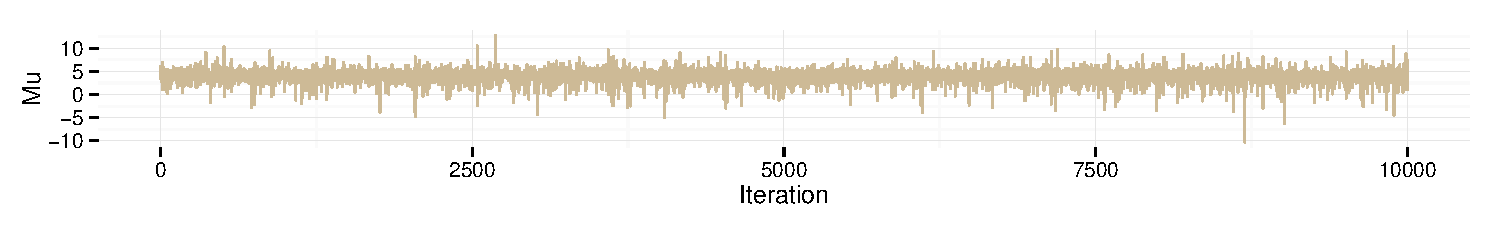
\includegraphics{markdown_hw3_files/figure-latex/unnamed-chunk-7-1.pdf}
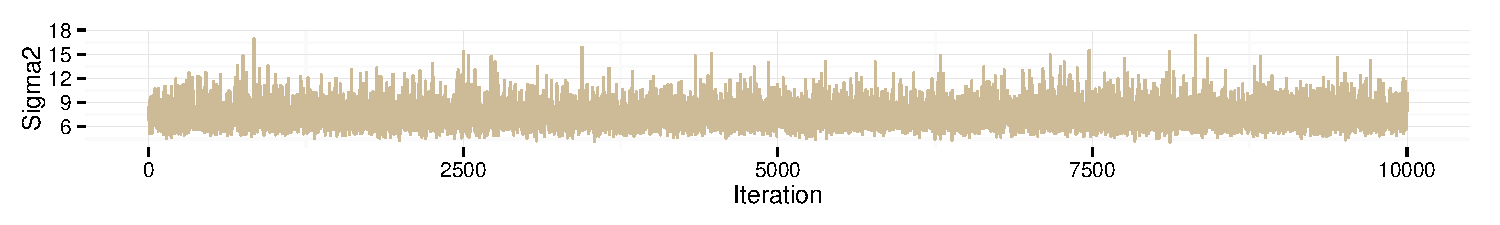
\includegraphics{markdown_hw3_files/figure-latex/unnamed-chunk-8-1.pdf}
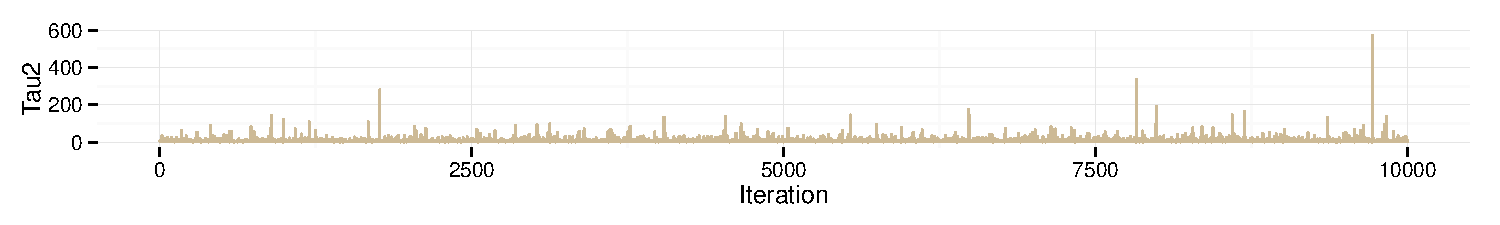
\includegraphics{markdown_hw3_files/figure-latex/unnamed-chunk-8-2.pdf}
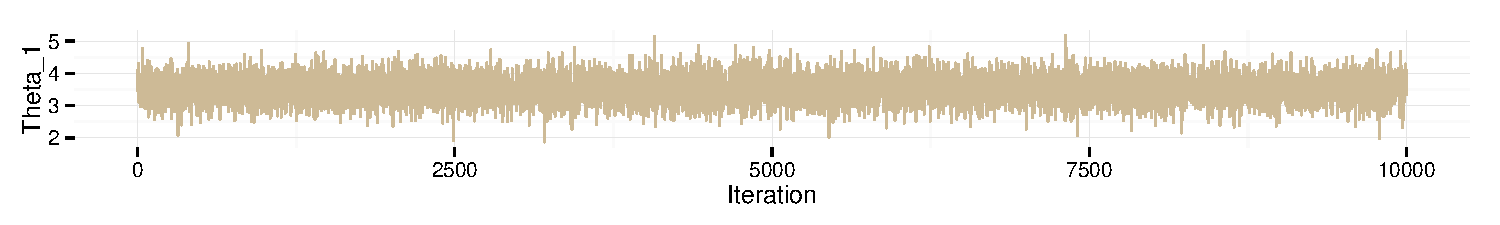
\includegraphics{markdown_hw3_files/figure-latex/unnamed-chunk-8-3.pdf}
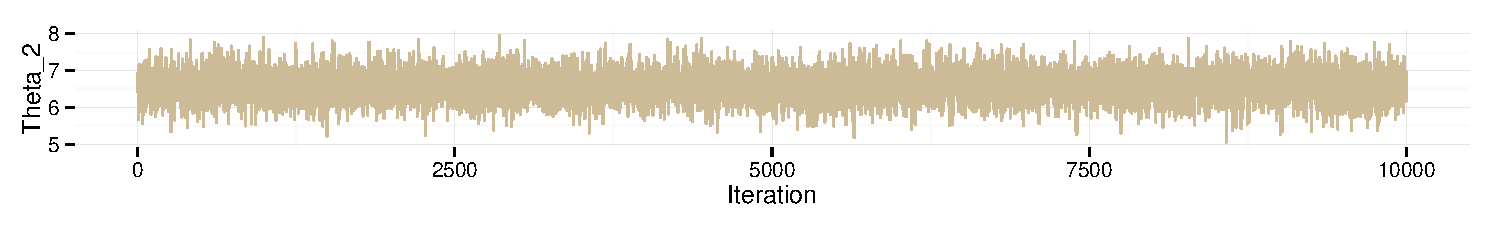
\includegraphics{markdown_hw3_files/figure-latex/unnamed-chunk-8-4.pdf}
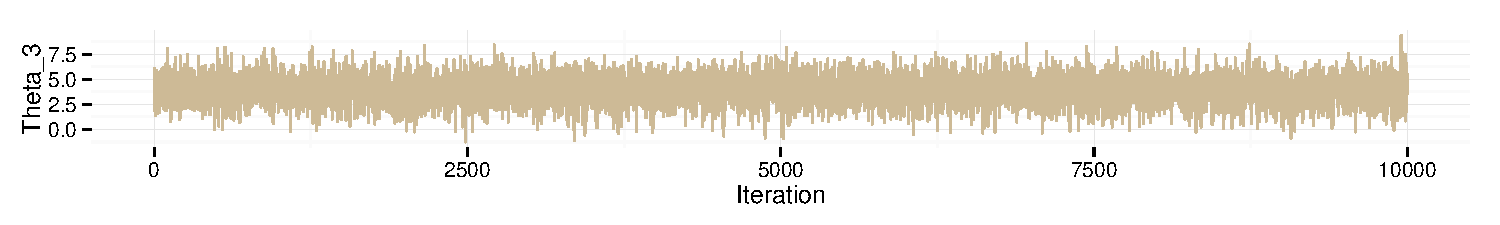
\includegraphics{markdown_hw3_files/figure-latex/unnamed-chunk-8-5.pdf}
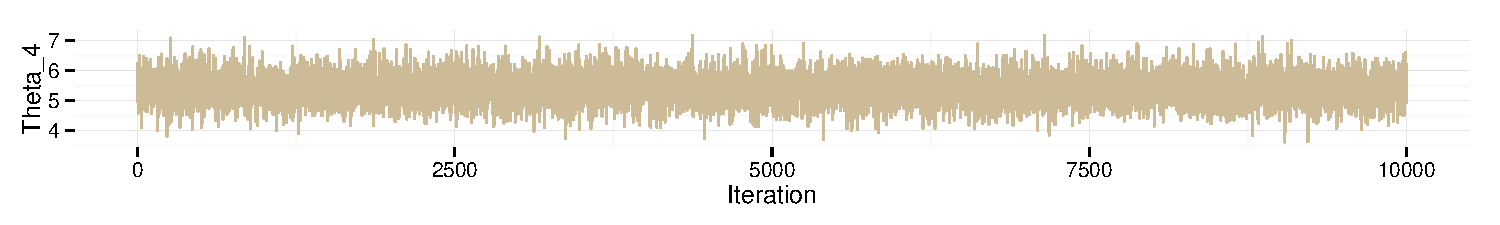
\includegraphics{markdown_hw3_files/figure-latex/unnamed-chunk-8-6.pdf}
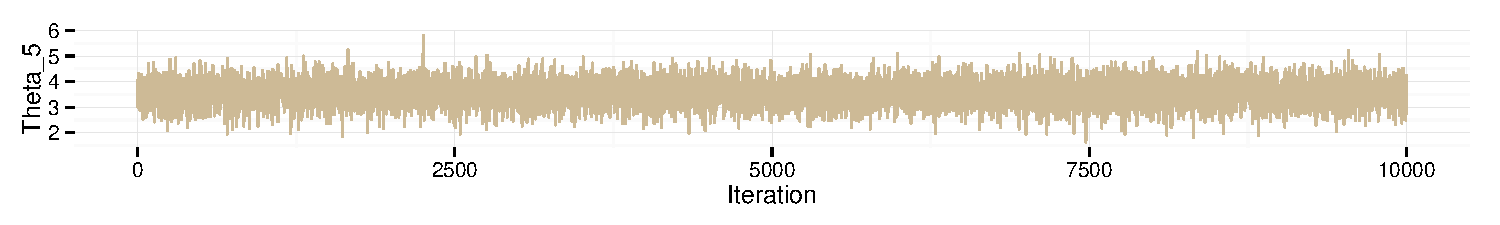
\includegraphics{markdown_hw3_files/figure-latex/unnamed-chunk-8-7.pdf}

We conclude from the graphs that convergence was achieved for all
parameters.

\subsection{1.3 Algorithm output}

The estimated median values and 95\% credible intervals for the
parameters are as follow:

\begin{Shaded}
\begin{Highlighting}[]
  \NormalTok{for(i in }\DecValTok{1}\NormalTok{:}\KeywordTok{length}\NormalTok{(ALL[}\DecValTok{1}\NormalTok{,])) }\KeywordTok{print}\NormalTok{(}\KeywordTok{round}\NormalTok{(}\KeywordTok{unname}\NormalTok{(}
    \KeywordTok{quantile}\NormalTok{(ALL[,i], }\DataTypeTok{probs=}\KeywordTok{c}\NormalTok{(}\FloatTok{0.025}\NormalTok{, }\FloatTok{0.5}\NormalTok{, }\FloatTok{0.975}\NormalTok{))}
    \NormalTok{),}\DecValTok{3}\NormalTok{))}
\end{Highlighting}
\end{Shaded}

\begin{center}
  \begin{tabular}{l c c c}
  \hline Parameter & Credible Lower 95\% & Median & Credible Upper 95\%  \\ \hline
    $\theta_1$ (Basmati) & 2.810 & 3.569 & 4.308 \\ 
    $\theta_2$ (Non-Basmati) & 5.790 & 6.533 & 7.305 \\
    $\theta_3$ (Beverage) & 1.869 & 4.231 & 6.448 \\
    $\theta_4$ (Cakes) & 4.486 & 5.370 & 6.301 \\
    $\theta_5$ (Cereal) & 2.705 & 3.610 & 4.507 \\
    $\mu$ & 3.193 & 4.697 & 6.182 \\
    $\sigma^2$ & 5.109 & 7.027 & 10.573 \\
    $\tau^2$ & 0.693 &2.251 & 12.920 \\ \hline
  \end{tabular}
\end{center}

\subsection{1.4 Sensitivity analyses}

Evaluation of sensitivity to priors: we try three separate scenarios
each tuning prior distribution of parameters:

\begin{enumerate}
  \item Large expected $\mu$ (Prior expectation of mad levels of arsenic)
  \item Large $\sigma^2$ and $\nu_0$ (High variability within products)
  \item Large $\tau^2$ and $\eta_0$ (High variability between products)
\end{enumerate}

\textit{Scenario 1}:

\begin{center}
  \begin{tabular}{l c c c}
  \hline Parameter & Credible Lower 95\% & Median & Credible Upper 95\%  \\ \hline
    $\theta_1$ (Basmati)&2.706&3.488&4.265\\
    $\theta_2^2$ (Non-Basmati)&5.902&6.671&7.460\\
    $\theta_3 (Beverage)$&0.643&3.774&6.932\\
    $\theta_4 (Cakes)$&4.511&5.452&6.429\\
    $\theta_5$ (Cereal)&2.548&3.496&4.456\\
    $\mu$ &2.548&3.496&4.456\\
    $\sigma^2$ &88.793&100&111\\
    $\tau^2$ &3021.927&8427&37962\\ \hline
  \end{tabular}
\end{center}

\textit{Scenario 2}:

\begin{center}
  \begin{tabular}{l c c c}
  \hline Parameter & Credible Lower 95\% & Median & Credible Upper 95\% \\ \hline
    $\theta_1$ (Basmati)& 1.237 & 4.396 & 7.069\\
    $\theta_2^2$ (Non-Basmati)& 2.811 & 5.401 & 8.559 \\
    $\theta_3 (Beverage)$& 0.278 & 4.790 & 9.023 \\
    $\theta_4 (Cakes)$& 1.931 & 4.960 & 8.221\\
    $\theta_5$ (Cereal)& 1.137 & 4.531 & 7.508\\
    $\mu$ &2.42 & 4.84 & 7.19\\
    $\sigma^2$ &182 & 215& 256\\
    $\tau^2$ &0.399 & 1.876 & 22.3\\ \hline

  \end{tabular}
\end{center}

\textit{Scenario 3}:

\begin{center}
  \begin{tabular}{l c c c}
  \hline Parameter & Credible Lower 95\% & Median & Credible Upper 95\% \\ \hline
    $\theta_1$ (Basmati)& 2.707 & 3.478 & 4.268\\
    $\theta_2^2$ (Non-Basmati)& 5.907 & 6.674 & 7.451 \\
    $\theta_3 (Beverage)$& 0.676 & 3.739 & 6.9023 \\
    $\theta_4 (Cakes)$& 4.504 & 5.447 & 6.419\\
    $\theta_5$ (Cereal)& 2.547 & 3.494 & 4.452\\
    $\mu$ &-5.302 & 4.845 & 5.00\\
    $\sigma^2$ &5.197 & 7.327 & 11.37\\
    $\tau^2$ &223 & 288 & 384\\ \hline
  \end{tabular}
\end{center}

We observe that excessively large prior expectations of \(\mu\) will
drive up estimates of the within- and between-group variances but will
have little effect on the magnitude of the estimates of within-groupmean
estimates (although the precision may be negatively affected for groups
with realtively few observations). A large prior within-sample variance
will bring posterior within-group means closer to \(\mu\), as could be
expected since the posterior estimates need to become more conservative.
Increasing prior between-sample variance appears to drive up uncertainty
on \(\mu\) and bring it closer to \(0\), without however having a
notable impact on the rest of the model.

\subsection{1.5 Results presentation}

Non-Basmati rice had the highest arsenic concentration, at an estimated
6.7 mcg/serving. Rice cakes came second, at 5.4 mcg/serving, and
non-Basmati and rice cereal had comparatively low amounts, slightly
below 3.5 mcg/serving. There lacked data to reliably evaluate arsenic
concentration in rice beverages, whose 3.8 mcg/serving estimate was
particulary imprecise (95\% CI=0.64, 6.93). Posterior median estimates
and observed mean concentrations of arsenic are presented by product
type in the following graph. Markers are \(\theta\) estimates with
\(95\%\) credible interval lines; horizontal lines are the median
estimate of \(\mu\) (solid) and corresponding \(95\%\) credibal interval
(dashed).

\begin{Shaded}
\begin{Highlighting}[]
\NormalTok{qmat=}\KeywordTok{apply}\NormalTok{(THETA[,}\DecValTok{1}\NormalTok{:}\DecValTok{5}\NormalTok{],}\DecValTok{2}\NormalTok{,quantile,}\DataTypeTok{probs=}\KeywordTok{c}\NormalTok{(}\FloatTok{0.025}\NormalTok{,.}\DecValTok{5}\NormalTok{,}\FloatTok{0.975}\NormalTok{))}
\NormalTok{mu_ci =}\StringTok{ }\KeywordTok{quantile}\NormalTok{(OTH[,}\DecValTok{1}\NormalTok{], }\DataTypeTok{probs=}\NormalTok{(}\KeywordTok{c}\NormalTok{(}\FloatTok{0.025}\NormalTok{, }\FloatTok{0.5}\NormalTok{, }\FloatTok{0.975}\NormalTok{)))}
\NormalTok{res <-}\StringTok{ }\KeywordTok{data.frame}\NormalTok{(}\StringTok{"Rice"}\NormalTok{=}\KeywordTok{c}\NormalTok{(}\StringTok{"Non-Basmati"}\NormalTok{, }\StringTok{"Basmati"}\NormalTok{, }\StringTok{"Beverages"}\NormalTok{, }\StringTok{"Cakes"}\NormalTok{, }\StringTok{"Cereal"}\NormalTok{),}
                         \StringTok{"l95"}\NormalTok{=qmat[}\DecValTok{1}\NormalTok{,], }\StringTok{"median"}\NormalTok{=qmat[}\DecValTok{2}\NormalTok{,], }\StringTok{"u95"}\NormalTok{=qmat[}\DecValTok{3}\NormalTok{,], }\StringTok{"mean"}\NormalTok{=ybar)}
\NormalTok{g <-}\StringTok{ }\KeywordTok{ggplot}\NormalTok{(res, }\KeywordTok{aes}\NormalTok{(}\DataTypeTok{x =} \NormalTok{Rice, }\DataTypeTok{group=}\NormalTok{Rice, }\DataTypeTok{colour=}\NormalTok{Rice)) +}\StringTok{ }
\StringTok{  }\KeywordTok{labs}\NormalTok{(}\DataTypeTok{x=}\StringTok{"Rice Products"}\NormalTok{, }\DataTypeTok{y=}\StringTok{"Arsenic concentration, mcg/serving"}\NormalTok{) +}\StringTok{ }
\StringTok{  }\KeywordTok{theme}\NormalTok{(}\DataTypeTok{legend.position=}\StringTok{"none"}\NormalTok{, }\DataTypeTok{panel.background =}\KeywordTok{element_rect}\NormalTok{(}\DataTypeTok{colour =} \StringTok{"black"}\NormalTok{)) +}
\StringTok{  }\KeywordTok{scale_y_continuous}\NormalTok{(}\DataTypeTok{breaks=}\KeywordTok{seq}\NormalTok{(}\DecValTok{0}\NormalTok{, }\FloatTok{7.5}\NormalTok{, }\DecValTok{1}\NormalTok{)) +}
\StringTok{  }\KeywordTok{geom_hline}\NormalTok{(}\KeywordTok{aes}\NormalTok{(}\DataTypeTok{yintercept=}\KeywordTok{c}\NormalTok{(mu_ci[}\DecValTok{2}\NormalTok{])), }\DataTypeTok{size=}\FloatTok{0.7}\NormalTok{) +}
\StringTok{  }\KeywordTok{geom_hline}\NormalTok{(}\KeywordTok{aes}\NormalTok{(}\DataTypeTok{yintercept=}\KeywordTok{c}\NormalTok{(mu_ci[}\DecValTok{1}\NormalTok{])), }\DataTypeTok{linetype=}\StringTok{"dashed"}\NormalTok{) +}
\StringTok{  }\KeywordTok{geom_hline}\NormalTok{(}\KeywordTok{aes}\NormalTok{(}\DataTypeTok{yintercept=}\KeywordTok{c}\NormalTok{(mu_ci[}\DecValTok{3}\NormalTok{])), }\DataTypeTok{linetype=}\StringTok{"dashed"}\NormalTok{) +}
\StringTok{  }\KeywordTok{geom_errorbar}\NormalTok{(}\KeywordTok{aes}\NormalTok{(}\DataTypeTok{ymin=}\NormalTok{l95, }\DataTypeTok{ymax=}\NormalTok{u95), }\DataTypeTok{width=}\NormalTok{.}\DecValTok{3}\NormalTok{, }\DataTypeTok{size=}\FloatTok{0.8}\NormalTok{) +}
\StringTok{  }\KeywordTok{geom_point}\NormalTok{(}\KeywordTok{aes}\NormalTok{(}\DataTypeTok{y=}\NormalTok{median), }\DataTypeTok{fill=}\StringTok{"white"}\NormalTok{, }\DataTypeTok{shape=}\DecValTok{21}\NormalTok{, }\DataTypeTok{size=}\DecValTok{5}\NormalTok{)  +}
\StringTok{  }\KeywordTok{geom_point}\NormalTok{(}\KeywordTok{aes}\NormalTok{(}\DataTypeTok{y=}\NormalTok{mean), }\DataTypeTok{fill=}\StringTok{"red"}\NormalTok{, }\DataTypeTok{shape=}\DecValTok{21}\NormalTok{, }\DataTypeTok{size=}\DecValTok{3}\NormalTok{)}
\NormalTok{g}
\end{Highlighting}
\end{Shaded}

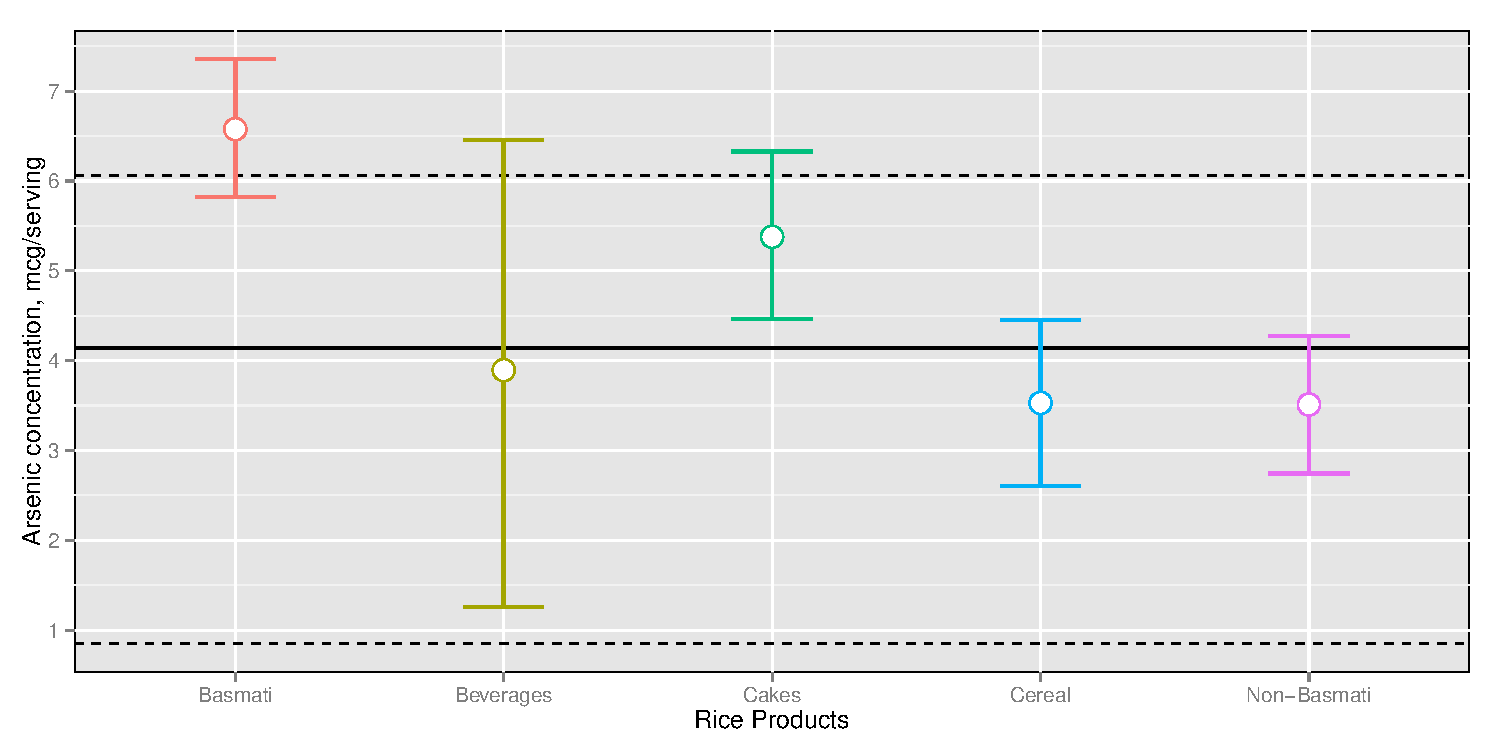
\includegraphics{markdown_hw3_files/figure-latex/unnamed-chunk-10-1.pdf}
\newpage \section{2. Parameter-expanded specification of the hierarchical model}
\subsection{2.1 Model specification} Under this model specification,
instead of group means we are interested in differences between groups
and the population average \(\mu\), which is given by \(\eta_j\) for the
group \(j\), so that (under the prior belief that all groups will have
equal mean):

\begin{align*}
  y_{ij} \sim& \, \mathcal{N}\left( \mu + \xi\eta_j, \sigma_y^2 \right)\\
  \eta_i \sim& \, \mathcal{N}\left( 0, \sigma_\eta^2 \right)
\end{align*}

Word's on the street that well-behaved conditionally-conjugate
specifications for the distributions of \(\xi\) and \(\sigma_\eta^2\)
are:

\begin{align*}
  \xi \sim& \, \mathcal{N}\left( 0, 1 \right) \\
  1/\sigma^2_\eta \sim& \, \text{gamma}\left( \frac{\omega_0}{2}, \frac{\omega_0\sigma^2_{\eta0}}{2} \right) \\
  1/\sigma^2_y \sim& \, \text{gamma}\left( \frac{\nu_0}{2}, \frac{\nu_0\sigma^2_{y0}}{2}\right)
\end{align*}

The prior distribution of the population mean is still
\(\mu \sim \, \mathcal{N}\left( \mu_0, \gamma_0^2\right)\). We set out
to find full conditionals: Reparametrizing the full conditionals in
exercise 1 easily yields what we need: \newline

Note that each of the \(N\) observation in the data supports,
\(\mu = y_{ij} - xi\eta_j\) given known \(\xi\) and \(\eta_j\)'s, so
that, summing over this expression and weighting it against the prior
yields:

\begin{flalign*}
p\left( \mu, \sigma^2_y, \sigma^2_\eta, \xi, \eta_1,\ldots,\eta_m \, | \, \mathbf{y}\right) \alpha& \; \mathcal{N} \left( \frac{\frac{\sum\limits_j\sum\limits_i y_{ij} - \xi\eta_j}{\sigma^2_y} + \frac{\mu_0}{\gamma_0^2}}{\frac{N}{\sigma^2_y}+\frac{1}{\gamma_0^2}},\frac{1}{\frac{N}{\sigma^2_y}+\frac{1}{\gamma_0^2}} \right) &
\end{flalign*}

Posterior on the variances can be similarly rewritten. The sum of
squares for \(\mathbf{y}\) given \(\mu, \eta_j\) and \(\xi\) is, of
course, \(\sum\limits_j\sum\limits_i y_{ij} - \mu - \xi\eta_j\), and the
sum of squares of \(\boldsymbol{\eta}\) given its \(\mathbb{E}=0\) is
simply \(\sum\limits_j\eta_j^2\)

\begin{flalign*}
p\left( 1/\sigma^2_y \, | \, \mathbf{y}, \mu, \sigma^2_\eta, \xi, \eta_1,\ldots,\eta_m \right) \alpha& \; \text{gamma }\left( \frac{\nu_0 + N}{2}, \frac{1}{2}\left( \nu_0\sigma_{y0}^2 + \sum\limits_j\sum\limits_i \left(y_{ij} - \mu - \xi\eta_j \right)^2 \right) \right) & \\
p\left( 1/\sigma^2_\eta \, | \, \mathbf{y}, \mu, \sigma^2_y, \xi, \eta_1,\ldots,\eta_m \right) \alpha& \; \text{gamma }\left( \frac{\omega_0 + m}{2}, \frac{1}{2}\left( \omega_0\sigma_{\eta_0}^2 + \sum\limits_j\eta_j^2 \right) \right)  &
\end{flalign*}

Getting full conditionals on \(\boldsymbol{\eta}\) and \(\xi\) can be
likewise achieved by manipulating \(y_{ij} = \mu + \eta_j\xi\).

\begin{flalign*}
  p\left( \eta_j \, | \, \mathbf{y}, \mu, \sigma^2_y, \sigma^2_\eta, \xi \right) \alpha& \; \mathcal{N}\left( \frac{\frac{\xi\sum\limits_iy_{ij}-\mu}{\sigma^2_y}}{\frac{n_j\xi^2}{\sigma^2_y}+\frac{1}{\sigma^2_\eta}}, \frac{1}{{\frac{n_j\xi^2}{\sigma^2_y}+\frac{1}{\sigma^2_\eta}}}\right) & 
\end{flalign*}

and

\begin{flalign*}
  p\left( \xi \, | \, \mathbf{y}, \mu, \sigma^2_y, \sigma^2_\eta, \eta_1,\ldots,\eta_m \right) \alpha& \; \mathcal{N} \left( \frac{\frac{\sum\limits_j\eta_j\sum\limits_i \left( y_{ij} - \mu \right)}{\sigma^2_y}}{\frac{\sum\limits_j n_j \eta_j^2}{\sigma^2_y}+1}, \frac{1}{\frac{\sum\limits_j n_j \eta_j^2}{\sigma^2_y}+1}\right) &
\end{flalign*}\subsection{2.2 Analyses}

Similarly to exercise 1, we pick the priors
\(\sigma^2_{y0} = 10, \nu_0 = 1, \omega_0 = 1, \sigma_{0\eta}^2 = 10\)
and \(\gamma_0^2 = 10\), and proceed with Gibbs sampling:

We read the data

\begin{Shaded}
\begin{Highlighting}[]
\KeywordTok{library}\NormalTok{(foreign)}
\KeywordTok{library}\NormalTok{(hdrcde)}
\end{Highlighting}
\end{Shaded}

\begin{verbatim}
## Loading required package: mvtnorm
## hdrcde 3.1 loaded
\end{verbatim}

\begin{Shaded}
\begin{Highlighting}[]
\NormalTok{data <-}\StringTok{ }\KeywordTok{read.dta}\NormalTok{(}\DataTypeTok{file=}\StringTok{"arsenicrice2.dta"}\NormalTok{)}
\NormalTok{Y <-}\StringTok{ }\KeywordTok{read.dta}\NormalTok{(}\DataTypeTok{file=}\StringTok{"arsenicrice2.dta"}\NormalTok{)}
\end{Highlighting}
\end{Shaded}

We set prior values

\begin{Shaded}
\begin{Highlighting}[]
\NormalTok{n <-}\StringTok{  }\KeywordTok{nrow}\NormalTok{(Y)}
\NormalTok{nu0 <-}\StringTok{ }\DecValTok{1}\NormalTok{; omega0 <-}\StringTok{ }\DecValTok{1}\NormalTok{; }
\NormalTok{s2_eta0 <-}\StringTok{ }\DecValTok{10}\NormalTok{; s2_y0 <-}\StringTok{ }\DecValTok{10}
\NormalTok{mu0 <-}\StringTok{ }\KeywordTok{mean}\NormalTok{(Y$arsenic); }
\NormalTok{g20 <-}\StringTok{ }\KeywordTok{var}\NormalTok{(Y$arsenic)}
\end{Highlighting}
\end{Shaded}

We setup the MCMC

\begin{Shaded}
\begin{Highlighting}[]
\CommentTok{#Setup starting values }
\NormalTok{m <-}\StringTok{ }\KeywordTok{length}\NormalTok{(}\KeywordTok{unique}\NormalTok{(Y$food_num)) }\CommentTok{#number of groups}
\NormalTok{n <-}\StringTok{ }\NormalTok{sv_y <-}\StringTok{ }\NormalTok{ybar <-}\StringTok{ }\KeywordTok{rep}\NormalTok{(}\OtherTok{NA}\NormalTok{,m) }\CommentTok{#create empty vectors for group descriptions}
\NormalTok{for (i in }\DecValTok{1}\NormalTok{:m) }
\NormalTok{\{}
  \NormalTok{n[i] <-}\StringTok{ }\KeywordTok{sum}\NormalTok{(Y$food_num==i)}
  \NormalTok{sv_y[i] <-}\StringTok{ }\KeywordTok{var}\NormalTok{(Y$arsenic[}\KeywordTok{which}\NormalTok{(Y$food_num==i)])}
  \NormalTok{ybar[i] <-}\StringTok{  }\KeywordTok{mean}\NormalTok{(Y$arsenic[}\KeywordTok{which}\NormalTok{(Y$food_num==i)])}
\NormalTok{\}}
\NormalTok{eta <-}\StringTok{ }\NormalTok{ybar -}\StringTok{ }\KeywordTok{mean}\NormalTok{(Y$arsenic); s2_y <-}\StringTok{ }\KeywordTok{mean}\NormalTok{(sv_y)}
\NormalTok{mu <-}\StringTok{ }\KeywordTok{mean}\NormalTok{(Y$arsenic); s2_eta <-}\StringTok{ }\KeywordTok{var}\NormalTok{(eta)}
\NormalTok{xi <-}\StringTok{ }\DecValTok{0}

\CommentTok{#Setup MCMC}
\KeywordTok{set.seed}\NormalTok{(}\DecValTok{0808}\NormalTok{)}
\NormalTok{S <-}\StringTok{ }\DecValTok{10000}
\NormalTok{THETA <-}\StringTok{ }\KeywordTok{matrix}\NormalTok{(}\DataTypeTok{nrow=}\NormalTok{S, }\DataTypeTok{ncol=}\NormalTok{m)}
\NormalTok{RES <-}\StringTok{ }\KeywordTok{matrix}\NormalTok{(}\DataTypeTok{nrow=}\NormalTok{S, }\DataTypeTok{ncol=}\DecValTok{4}\NormalTok{)}
\NormalTok{ALL <-}\StringTok{ }\KeywordTok{matrix}\NormalTok{(}\DataTypeTok{nrow=}\NormalTok{S, }\DataTypeTok{ncol=}\DecValTok{4}\NormalTok{+m)}

\CommentTok{#Setup MCMC}
\KeywordTok{set.seed}\NormalTok{(}\DecValTok{0808}\NormalTok{)}
\NormalTok{S <-}\StringTok{ }\DecValTok{10000}
\NormalTok{ETA <-}\StringTok{ }\KeywordTok{matrix}\NormalTok{(}\DataTypeTok{nrow=}\NormalTok{S, }\DataTypeTok{ncol=}\NormalTok{m)}
\NormalTok{RES <-}\StringTok{ }\KeywordTok{matrix}\NormalTok{(}\DataTypeTok{nrow=}\NormalTok{S, }\DataTypeTok{ncol=}\DecValTok{4}\NormalTok{)}
\NormalTok{ALL <-}\StringTok{ }\KeywordTok{matrix}\NormalTok{(}\DataTypeTok{nrow=}\NormalTok{S, }\DataTypeTok{ncol=}\DecValTok{4}\NormalTok{+m)}
\end{Highlighting}
\end{Shaded}

Our updating functions correspond to the full conditionals derived
above:

\begin{Shaded}
\begin{Highlighting}[]
\CommentTok{#FUNCTIONS}
\NormalTok{newS2eta <-}\StringTok{ }\NormalTok{function(m, s2_eta0, eta, omega0)}
\NormalTok{\{}
  \NormalTok{ss <-}\StringTok{ }\NormalTok{s2_eta0*omega0 +}\StringTok{ }\KeywordTok{sum}\NormalTok{( eta^}\DecValTok{2} \NormalTok{)}
  \NormalTok{s2_eta <-}\StringTok{ }\DecValTok{1}\NormalTok{/}\KeywordTok{rgamma}\NormalTok{(}\DecValTok{1}\NormalTok{, }\DataTypeTok{shape=}\NormalTok{((omega0 +}\StringTok{ }\NormalTok{m)/}\DecValTok{2}\NormalTok{), }\DataTypeTok{scale=}\NormalTok{(ss/}\DecValTok{2}\NormalTok{))}
  \KeywordTok{return}\NormalTok{(s2_eta)}
\NormalTok{\}}
\NormalTok{newS2y <-}\StringTok{ }\NormalTok{function(nu0, n, s2_y0, y, m, eta, xi, mu)}
\NormalTok{\{}
  \NormalTok{nun =}\StringTok{ }\NormalTok{nu0 +}\StringTok{ }\KeywordTok{sum}\NormalTok{(n)}
  \NormalTok{ss =}\StringTok{ }\KeywordTok{sum}\NormalTok{((y -}\StringTok{ }\NormalTok{mu -}\StringTok{ }\NormalTok{xi*}\KeywordTok{rep}\NormalTok{(eta, }\DataTypeTok{times=}\NormalTok{n))^}\DecValTok{2}\NormalTok{) +}\StringTok{ }\NormalTok{nu0*s2_y0}
  \NormalTok{s2_y <-}\StringTok{ }\DecValTok{1}\NormalTok{/}\KeywordTok{rgamma}\NormalTok{(}\DecValTok{1}\NormalTok{, }\DataTypeTok{shape=}\NormalTok{(nun/}\DecValTok{2}\NormalTok{), }\DataTypeTok{scale=}\NormalTok{(ss/}\DecValTok{2}\NormalTok{))}
  \KeywordTok{return}\NormalTok{(s2_y)}
\NormalTok{\}}
\NormalTok{newMu <-}\StringTok{ }\NormalTok{function(y, xi, eta, s2_y, g20, mu0, n)}
\NormalTok{\{}
  \NormalTok{v =}\StringTok{ }\NormalTok{( }\KeywordTok{sum}\NormalTok{(n)/s2_y +}\StringTok{ }\DecValTok{1}\NormalTok{/g20 )}
  \NormalTok{ss =}\StringTok{ }\KeywordTok{sum}\NormalTok{(y-}\KeywordTok{rep}\NormalTok{(eta,}\DataTypeTok{times=}\NormalTok{n)*xi)/s2_y +}\StringTok{ }\NormalTok{mu0/g20}
  \NormalTok{e =}\StringTok{ }\NormalTok{(ss/s2_y +}\StringTok{ }\NormalTok{mu0/g20)}
  \NormalTok{mu =}\StringTok{ }\KeywordTok{rnorm}\NormalTok{(}\DecValTok{1}\NormalTok{, ss/v, }\KeywordTok{sqrt}\NormalTok{(}\DecValTok{1}\NormalTok{/v))}
  \KeywordTok{return}\NormalTok{(mu)}
\NormalTok{\}}
\NormalTok{newEta <-}\StringTok{ }\NormalTok{function(xi, mu, ybar, n, s2_y, s2_eta)}
\NormalTok{\{}
  \NormalTok{v =}\StringTok{ }\DecValTok{1}\NormalTok{/(n*xi^}\DecValTok{2}\NormalTok{/s2_y +}\StringTok{ }\DecValTok{1}\NormalTok{/s2_eta)}
  \NormalTok{e =}\StringTok{ }\NormalTok{v*xi*(n*ybar -}\StringTok{ }\NormalTok{mu*n)/s2_y}
  \NormalTok{eta =}\StringTok{ }\KeywordTok{rnorm}\NormalTok{(m, e, }\KeywordTok{sqrt}\NormalTok{(v))}
  \KeywordTok{return}\NormalTok{(eta)}
\NormalTok{\}}
\NormalTok{newXi <-}\StringTok{ }\NormalTok{function(eta, m, y, n, mu, s2_y)}
\NormalTok{\{}
  \NormalTok{v =}\StringTok{ }\NormalTok{(}\KeywordTok{sum}\NormalTok{(n*eta^}\DecValTok{2}\NormalTok{)/s2_y +}\StringTok{ }\DecValTok{1}\NormalTok{)}
  \NormalTok{e =}\StringTok{ }\KeywordTok{sum}\NormalTok{((y-mu)*}\KeywordTok{rep}\NormalTok{(eta,}\DataTypeTok{times=}\NormalTok{n))/s2_y}
  \NormalTok{xi =}\StringTok{ }\KeywordTok{rnorm}\NormalTok{(}\DecValTok{1}\NormalTok{, e/v, }\KeywordTok{sqrt}\NormalTok{(}\DecValTok{1}\NormalTok{/v))}
  \KeywordTok{return}\NormalTok{(xi)}
\NormalTok{\}}
\end{Highlighting}
\end{Shaded}

We run the MCMC algorithm:

\begin{Shaded}
\begin{Highlighting}[]
\CommentTok{#RUN MCMC}
\NormalTok{for(i in }\DecValTok{1}\NormalTok{:S)}
\NormalTok{\{}
  \CommentTok{#Get new values for parameters}
  \NormalTok{eta <-}\StringTok{ }\KeywordTok{newEta}\NormalTok{(xi, mu, ybar, n, s2_y, s2_eta)}
  \NormalTok{mu <-}\StringTok{ }\KeywordTok{newMu}\NormalTok{(Y$arsenic, xi, eta, s2_y, g20, mu0, n)}
  
  \NormalTok{s2_eta <-}\StringTok{ }\KeywordTok{newS2eta}\NormalTok{(m, s2_eta0, eta, omega0)}
  \NormalTok{s2_y <-}\StringTok{ }\KeywordTok{newS2y}\NormalTok{(nu0, n, s2_y0, Y$arsenic, m, eta, xi, mu)}
  
  \NormalTok{xi <-}\StringTok{ }\KeywordTok{newXi}\NormalTok{(eta, m, Y$arsenic, n, mu, s2_y)}
  \CommentTok{#Store in chain}
  \NormalTok{ETA[i,] <-}\StringTok{ }\NormalTok{eta}
  \NormalTok{RES[i,] <-}\StringTok{ }\KeywordTok{c}\NormalTok{(mu,s2_y, s2_eta, xi)}
  \NormalTok{ALL[i,] <-}\StringTok{ }\KeywordTok{c}\NormalTok{(eta, mu, xi, s2_eta, s2_y)}
\NormalTok{\}}
\end{Highlighting}
\end{Shaded}

Again, before we get too psyched about results, we check MCMC
convergence criteria (code not shown, see above):

\includegraphics{markdown_hw3_files/figure-latex/unnamed-chunk-16-1.pdf}
\includegraphics{markdown_hw3_files/figure-latex/unnamed-chunk-16-2.pdf}
\includegraphics{markdown_hw3_files/figure-latex/unnamed-chunk-16-3.pdf}
\includegraphics{markdown_hw3_files/figure-latex/unnamed-chunk-16-4.pdf}
\includegraphics{markdown_hw3_files/figure-latex/unnamed-chunk-16-5.pdf}
\includegraphics{markdown_hw3_files/figure-latex/unnamed-chunk-16-6.pdf}
\includegraphics{markdown_hw3_files/figure-latex/unnamed-chunk-16-7.pdf}
\includegraphics{markdown_hw3_files/figure-latex/unnamed-chunk-16-8.pdf}
\includegraphics{markdown_hw3_files/figure-latex/unnamed-chunk-16-9.pdf}

Obviously, something is wrong with the \(\eta\) parameters, which could
make sense since when the estimate of \(\xi\) crosses zero, the \(\eta\)
parameters get updated on the other side of \(0\) as well. Taking the
absolute value of \(\xi\) reassures us that the parameter space that is
actually searched isn't terribad. We also check the convergence of
\(\mu + \xi\eta\), which is the mean concentration of arsenic in each
group, and ultimately interests us. Reproduced below are the graphs for
\(|\eta_1|, |\eta_2|\), and \(\boldsymbol{\theta}\)

\includegraphics{markdown_hw3_files/figure-latex/unnamed-chunk-17-1.pdf}
\includegraphics{markdown_hw3_files/figure-latex/unnamed-chunk-17-2.pdf}
\includegraphics{markdown_hw3_files/figure-latex/unnamed-chunk-17-3.pdf}
\includegraphics{markdown_hw3_files/figure-latex/unnamed-chunk-17-4.pdf}
\includegraphics{markdown_hw3_files/figure-latex/unnamed-chunk-17-5.pdf}
\includegraphics{markdown_hw3_files/figure-latex/unnamed-chunk-17-6.pdf}
\includegraphics{markdown_hw3_files/figure-latex/unnamed-chunk-17-7.pdf}
We are fairly satisfied with the outlook on the convergence of our
\(\theta\)'s, although obviously the wacky errors we'll get mean the
credible intervals we get for \(\theta\)'s will be meaningless.

\begin{figure}[h]
  \centering 
\includegraphics[width=0.7\textwidth]{hadeswrong}
  \caption{I know, Hades isn't pleased either}
\end{figure}\subsection{2.3 Algorithm output}

We provide the median estimate and 95\% credible interval for the
\(\theta\) parameters in this expanded hierarchical specification model:

\begin{center}
  \begin{tabular}{l c c c}
  \hline Parameter & Credible Lower 95\% & Median & Credible Upper 95\%  \\ \hline
    $\theta_1$ (Basmati) & 3.610 & 3.619 & 3.639 \\ 
    $\theta_2$ (Non-Basmati) & 6.420 & 6.454 & 6.503 \\
    $\theta_3$ (Beverage) & 4.072 & 4.361 & 4.544 \\
    $\theta_4$ (Cakes) & 5.308 & 5.331 & 5.345 \\
    $\theta_5$ (Cereal) & 3.649 & 3.670 & 3.747 \\ \hline
  \end{tabular}
\end{center}

\subsection{2.4 Sensitivity analyses}

We repeat the sensitivity analyses of section 1.4:

\begin{enumerate}
  \item Large expected $\mu$ (Prior expectation of mad levels of arsenic)
  \item Large $\sigma^2$ and $\nu_0$ (High variability within products)
  \item Large $\tau^2$ and $\eta_0$ (High variability between products)
\end{enumerate}

\textit{Scenario 1}:

\begin{center}
  \begin{tabular}{l c c c}
  \hline Parameter & Credible Lower 95\% & Median & Credible Upper 95\%  \\ \hline
    $\theta_1$ (Basmati) & 3.610 & 3.619 & 3.639 \\ 
    $\theta_2$ (Non-Basmati) & 6.421 & 6.454 & 6.503 \\
    $\theta_3$ (Beverage) & 4.072 & 4.361 & 4.544 \\
    $\theta_4$ (Cakes) & 5.308 & 5.332 & 5.345 \\
    $\theta_5$ (Cereal) & 3.649 & 3.670 & 3.747 \\ \hline
  \end{tabular}
\end{center}

\textit{Scenario 2}:

\begin{center}
  \begin{tabular}{l c c c}
  \hline Parameter & Credible Lower 95\% & Median & Credible Upper 95\%  \\ \hline
    $\theta_1$ (Basmati) & 3.610 & 3.619 & 3.639 \\ 
    $\theta_2$ (Non-Basmati) & 6.420 & 6.454 & 6.503 \\
    $\theta_3$ (Beverage) & 4.072 & 4.361 & 4.544 \\
    $\theta_4$ (Cakes) & 5.308 & 5.331 & 5.345 \\
    $\theta_5$ (Cereal) & 3.649 & 3.670 & 3.747 \\ \hline
  \end{tabular}
\end{center}

\textit{Scenario 3}:

\begin{center}
  \begin{tabular}{l c c c}
  \hline Parameter & Credible Lower 95\% & Median & Credible Upper 95\%  \\ \hline
    $\theta_1$ (Basmati) & 3.610 & 3.619 & 3.639 \\ 
    $\theta_2$ (Non-Basmati) & 6.420 & 6.454 & 6.503 \\
    $\theta_3$ (Beverage) & 4.072 & 4.361 & 4.544 \\
    $\theta_4$ (Cakes) & 5.308 & 5.331 & 5.345 \\
    $\theta_5$ (Cereal) & 3.649 & 3.670 & 3.747 \\ \hline
  \end{tabular}
\end{center}

We observe that outrageous standard errors will prevent any meaningful
sensitivity analyses.

\subsection{2.5 Results presentation}

Based on our analyses, and under the assumption we did nothing
incorrect, we are nearly positive that the type of rice with the
greatest arsenic concentration is non-basmati rice, at 6.420
mcg/serving, followed by cake rice products, at 5.308 mcg/serving.
Basmati and cereal products both neared 6.6mcg of arsening per serving,
beverage products, which should have constituted an imprecise estimate
(but did not), had an estimated arsenic concentration at 6.454
mcg/serving (95\% CI=4.361,4.544).

Posterior median estimates and observed mean concentrations of arsenic
are presented by product type in the following graph. Markers are
\(\theta\) estimates with \(95\%\) credible interval lines; horizontal
lines are the median estimate of \(\mu\) (solid) and corresponding
\(95\%\) credibal interval (dashed, like my hopes and dreams).

\includegraphics{markdown_hw3_files/figure-latex/unnamed-chunk-18-1.pdf}

\section{3. Conditionally-conjugate specification of the hierarchical model with group-specific variances}\subsection{3.1 Model specification}

This model is similar to that laid out in section 1.1, with the
exceptions that variance is allowed to vary between groups, with
group-specific variances following a conjugate inverse-gamma
distribution so that (from Hoff):

\begin{align*}
\left\{ \theta_j \, \left| \, \sigma^2, y_{j,1},\ldots,y_{j,n} \right. \right\} \sim& \, \mathcal{N}\left( \frac{n_j\bar{y}_j/\sigma^2+\mu/\tau^2}{n_j/\sigma^2 + 1/\tau^2}, \left[ n_j/\sigma^2+1/\tau^2\right]^{-1} \right) \\
    \left\{1/\sigma^2_j \, \left| \, \boldsymbol{\theta}, y_1, \ldots, y_n \right. \right\} \sim& \, \text{gamma}\left( \frac{1}{2}\left[ \nu_0 + n_j \right], \frac{1}{2}\left(\nu_0\sigma_0^2 + \sum\limits_{i=1}^{n_j} \left(y_{i,j} -\theta_j \right)^2 \right)\right) \\
    \left\{ \sigma^2_0 \left| \boldsymbol{\sigma}, \nu_0 \right. \right\} \sim& \, \text{gamma} \left( a + \frac{1}{2}m\nu_0, b + \frac{1}{2}\sum\limits_j\left( 1/\sigma^2_j \right) \right)
    \intertext{and}
    \left\{\nu_0 \left| \boldsymbol{\sigma} \right. \right\} \sim& \left( \frac{\left( \nu0\sigma_0^2/2\right)^{\nu_0/2}}{\Gamma\left( \nu_0/2\right)} \right)^m \left( \prod\limits_j\frac{1}{\sigma^2_j} \right)^{\nu_0/2-1} \times \exp\left\{ -\nu_0 \left( \alpha + \frac{1}{2} \sigma^2_0 \sum\limits_j \left( \frac{1}{\sigma^2_j}\right)\right) \right\}
\end{align*}\subsection{3.2 Analyses}

We keep the same priors for hyperparameters pertaining to \(\mu\) and
\(\theta\), and additionally specify \(\alpha = 1, b = 3, a = 1\) for
the prior distributions on \(\nu_0\) and \(\sigma^2_0\). Code to run
analyses is as follows, please refer to the earlier sections for added
description.

\begin{Shaded}
\begin{Highlighting}[]
\NormalTok{data <-}\StringTok{ }\KeywordTok{read.dta}\NormalTok{(}\DataTypeTok{file=}\StringTok{"arsenicrice2.dta"}\NormalTok{)}
\NormalTok{Y <-}\StringTok{ }\KeywordTok{read.dta}\NormalTok{(}\DataTypeTok{file=}\StringTok{"arsenicrice2.dta"}\NormalTok{)}

\CommentTok{#We set weakly informative prior values}
\NormalTok{n <-}\StringTok{  }\KeywordTok{nrow}\NormalTok{(Y)}
\NormalTok{eta0 <-}\StringTok{ }\DecValTok{1}\NormalTok{; t20 <-}\StringTok{ }\DecValTok{3}
\NormalTok{mu0 <-}\StringTok{ }\KeywordTok{mean}\NormalTok{(Y$arsenic) }
\NormalTok{g20  <-}\StringTok{ }\KeywordTok{var}\NormalTok{(Y$arsenic)}
\NormalTok{a =}\StringTok{ }\DecValTok{1}\NormalTok{; b =}\StringTok{ }\DecValTok{3}\NormalTok{; alpha =}\StringTok{ }\DecValTok{1}

\CommentTok{# mu0 <- 100 #scenario 1}
\CommentTok{# s20 <- 100*s20; nu0 <- 100 #scenario 2}
\CommentTok{# t20 <- 100*t20; eta0 <- 100 #scenario 3}
\CommentTok{#Setup starting values }

\NormalTok{m <-}\StringTok{ }\KeywordTok{length}\NormalTok{(}\KeywordTok{unique}\NormalTok{(Y$food_num)) }\CommentTok{#number of groups}
\NormalTok{n <-}\StringTok{ }\NormalTok{s2 <-}\StringTok{ }\NormalTok{ybar <-}\StringTok{ }\KeywordTok{rep}\NormalTok{(}\OtherTok{NA}\NormalTok{,m) }
\NormalTok{for (i in }\DecValTok{1}\NormalTok{:m) }
\NormalTok{\{}
  \NormalTok{n[i] <-}\StringTok{ }\KeywordTok{sum}\NormalTok{(Y$food_num==i)}
  \NormalTok{s2[i] <-}\StringTok{ }\KeywordTok{var}\NormalTok{(Y$arsenic[}\KeywordTok{which}\NormalTok{(Y$food_num==i)])}
  \NormalTok{ybar[i] <-}\StringTok{ }\KeywordTok{mean}\NormalTok{(Y$arsenic[}\KeywordTok{which}\NormalTok{(Y$food_num==i)])}
\NormalTok{\}}
\NormalTok{theta <-}\StringTok{ }\NormalTok{ybar; s2_0 <-}\StringTok{ }\KeywordTok{mean}\NormalTok{(sv)}
\NormalTok{mu <-}\StringTok{ }\KeywordTok{mean}\NormalTok{(theta); tau2 <-}\StringTok{ }\KeywordTok{var}\NormalTok{(theta)}
\NormalTok{nu0 <-}\StringTok{ }\DecValTok{1}

\CommentTok{#Setup MCMC}
\KeywordTok{set.seed}\NormalTok{(}\DecValTok{0808}\NormalTok{)}
\NormalTok{S <-}\StringTok{ }\DecValTok{10000}
\NormalTok{THETA2 <-}\StringTok{ }\NormalTok{S2 <-}\StringTok{ }\KeywordTok{matrix}\NormalTok{(}\DataTypeTok{nrow=}\NormalTok{S, }\DataTypeTok{ncol=}\NormalTok{m)}
\NormalTok{RES <-}\StringTok{ }\KeywordTok{matrix}\NormalTok{(}\DataTypeTok{nrow=}\NormalTok{S, }\DataTypeTok{ncol=}\DecValTok{4}\NormalTok{)}
\NormalTok{ALL <-}\StringTok{ }\KeywordTok{matrix}\NormalTok{(}\DataTypeTok{nrow=}\NormalTok{S, }\DataTypeTok{ncol=}\DecValTok{4+2}\NormalTok{*m)}
\NormalTok{NUMAX <-}\StringTok{ }\DecValTok{10000}

\NormalTok{### Functions sampling from posteriors}
\NormalTok{newTheta <-}\StringTok{ }\NormalTok{function(n, ybar, s2, tau2, mu)}
\NormalTok{\{}
  \NormalTok{v =}\StringTok{ }\DecValTok{1}\NormalTok{/(n/s2 +}\DecValTok{1}\NormalTok{/tau2)}
  \NormalTok{e =}\StringTok{ }\NormalTok{v *}\StringTok{ }\NormalTok{(ybar*n/s2 +}\StringTok{ }\NormalTok{mu/tau2)}
  \NormalTok{new <-}\StringTok{ }\KeywordTok{rnorm}\NormalTok{(}\KeywordTok{length}\NormalTok{(n), e, }\KeywordTok{sqrt}\NormalTok{(v))}
  \KeywordTok{return}\NormalTok{(new)}
\NormalTok{\}}
\NormalTok{newSigma2 <-}\StringTok{ }\NormalTok{function(m, n, nu0, s20, theta, y)}
\NormalTok{\{}
  \NormalTok{nun =}\StringTok{ }\NormalTok{n +}\StringTok{ }\NormalTok{nu0}
  \NormalTok{ss <-}\StringTok{ }\NormalTok{nu0 *}\StringTok{ }\NormalTok{s20 +}\StringTok{ }\KeywordTok{sum}\NormalTok{((y -}\StringTok{ }\KeywordTok{rep}\NormalTok{(theta, }\DataTypeTok{times=}\NormalTok{n))^}\DecValTok{2}\NormalTok{) }
  \NormalTok{sigma2 <-}\StringTok{ }\DecValTok{1}\NormalTok{/}\KeywordTok{rgamma}\NormalTok{(m, nun/}\DecValTok{2}\NormalTok{, ss/}\DecValTok{2}\NormalTok{)}
  \KeywordTok{return}\NormalTok{(sigma2)}
\NormalTok{\}}
\NormalTok{newMu <-}\StringTok{ }\NormalTok{function(m, theta, tau2, g20)}
\NormalTok{\{}
  \NormalTok{v =}\StringTok{ }\DecValTok{1}\NormalTok{/(m/tau2 +}\StringTok{ }\DecValTok{1}\NormalTok{/g20)}
  \NormalTok{e =}\StringTok{ }\NormalTok{v *(m*}\KeywordTok{mean}\NormalTok{(theta)/tau2 +}\StringTok{ }\NormalTok{mu0/g20)}
  \NormalTok{mu <-}\StringTok{ }\KeywordTok{rnorm}\NormalTok{(}\DecValTok{1}\NormalTok{, e, }\KeywordTok{sqrt}\NormalTok{(v))}
  \KeywordTok{return}\NormalTok{(mu)}
\NormalTok{\}}
\NormalTok{newTau2 <-}\StringTok{ }\NormalTok{function(m, eta0, t20, theta, mu)}
\NormalTok{\{}
  \NormalTok{etam =}\StringTok{ }\NormalTok{eta0 +}\StringTok{ }\NormalTok{m}
  \NormalTok{ss =}\StringTok{ }\NormalTok{eta0*t20 +}\StringTok{ }\KeywordTok{sum}\NormalTok{( (theta-mu) ^}\DecValTok{2} \NormalTok{)}
  \NormalTok{tau2 <-}\StringTok{ }\DecValTok{1}\NormalTok{/}\KeywordTok{rgamma}\NormalTok{(}\DecValTok{1}\NormalTok{, etam/}\DecValTok{2}\NormalTok{, ss/}\DecValTok{2}\NormalTok{)}
  \KeywordTok{return}\NormalTok{(tau2)}
\NormalTok{\}}
\NormalTok{newS20 <-}\StringTok{ }\NormalTok{function(m, nu0, s2, a, b)}
\NormalTok{\{}
  \NormalTok{L =}\StringTok{ }\NormalTok{a +}\StringTok{ }\FloatTok{0.5}\NormalTok{*m*nu0}
  \NormalTok{R =}\StringTok{ }\NormalTok{b +}\StringTok{ }\FloatTok{0.5}\NormalTok{*}\KeywordTok{sum}\NormalTok{(}\DecValTok{1}\NormalTok{/s2^}\DecValTok{2}\NormalTok{)}
  \NormalTok{s20 <-}\StringTok{ }\KeywordTok{rgamma}\NormalTok{(}\DecValTok{1}\NormalTok{, L, R)}
\NormalTok{\}}

\NormalTok{### Run MCMC}
\NormalTok{for(i in }\DecValTok{1}\NormalTok{:S)}
\NormalTok{\{}
  \CommentTok{#Get new values for parameters}
  \NormalTok{theta <-}\StringTok{ }\KeywordTok{newTheta}\NormalTok{(n, ybar, s2, tau2, mu)}
  \NormalTok{s2 <-}\StringTok{ }\KeywordTok{newSigma2}\NormalTok{(m, n, nu0, s20, theta, Y$arsenic)}
  \NormalTok{mu <-}\StringTok{ }\KeywordTok{newMu}\NormalTok{(m, theta, tau2, g20)}
  \NormalTok{tau2 <-}\StringTok{ }\KeywordTok{newTau2}\NormalTok{(m, eta0, t20, theta, mu)}
  \NormalTok{s20 <-}\StringTok{ }\KeywordTok{newS20}\NormalTok{(m, nu0, s2, a, b)}
  
  \NormalTok{x <-}\StringTok{ }\DecValTok{1}\NormalTok{:NUMAX}
    \NormalTok{lpnu0<-m*(.}\DecValTok{5}\NormalTok{*x*}\KeywordTok{log}\NormalTok{(s20*x/}\DecValTok{2}\NormalTok{)-}\KeywordTok{lgamma}\NormalTok{(x/}\DecValTok{2}\NormalTok{))+}
\StringTok{      }\NormalTok{(x/}\DecValTok{2-1}\NormalTok{)*}\KeywordTok{sum}\NormalTok{(}\KeywordTok{log}\NormalTok{(}\DecValTok{1}\NormalTok{/s2))+}
\StringTok{      }\NormalTok{-x*(alpha}\FloatTok{+.5}\NormalTok{*s20*}\KeywordTok{sum}\NormalTok{(}\DecValTok{1}\NormalTok{/s2))}
  \NormalTok{nu0<-}\KeywordTok{sample}\NormalTok{(x,}\DecValTok{1}\NormalTok{,}\DataTypeTok{prob=}\KeywordTok{exp}\NormalTok{(lpnu0-}\KeywordTok{max}\NormalTok{(lpnu0)))}
  
  
  \CommentTok{#Store in chain}
  \NormalTok{THETA2[i,] <-}\StringTok{ }\NormalTok{theta}
  \NormalTok{S2[i,] <-}\StringTok{ }\NormalTok{s2}
  \NormalTok{RES[i,] <-}\StringTok{ }\KeywordTok{c}\NormalTok{(mu,tau2, nu0, s20)}
  \NormalTok{ALL[i,] <-}\StringTok{ }\KeywordTok{c}\NormalTok{(theta,s2,mu,tau2, nu0, s20)}
\NormalTok{\}}
\end{Highlighting}
\end{Shaded}

Trace plots for the parameters follow:

\includegraphics{markdown_hw3_files/figure-latex/unnamed-chunk-20-1.pdf}
\includegraphics{markdown_hw3_files/figure-latex/unnamed-chunk-20-2.pdf}
\includegraphics{markdown_hw3_files/figure-latex/unnamed-chunk-20-3.pdf}
\includegraphics{markdown_hw3_files/figure-latex/unnamed-chunk-20-4.pdf}
\includegraphics{markdown_hw3_files/figure-latex/unnamed-chunk-20-5.pdf}
\includegraphics{markdown_hw3_files/figure-latex/unnamed-chunk-20-6.pdf}
\includegraphics{markdown_hw3_files/figure-latex/unnamed-chunk-20-7.pdf}
\includegraphics{markdown_hw3_files/figure-latex/unnamed-chunk-20-8.pdf}
\includegraphics{markdown_hw3_files/figure-latex/unnamed-chunk-20-9.pdf}
\includegraphics{markdown_hw3_files/figure-latex/unnamed-chunk-20-10.pdf}
\includegraphics{markdown_hw3_files/figure-latex/unnamed-chunk-20-11.pdf}
\includegraphics{markdown_hw3_files/figure-latex/unnamed-chunk-20-12.pdf}
\includegraphics{markdown_hw3_files/figure-latex/unnamed-chunk-20-13.pdf}
\includegraphics{markdown_hw3_files/figure-latex/unnamed-chunk-20-14.pdf}

Other than \(\sigma^2_3\) and \(\nu_0\), everything looks happy and
converged. \(\sigma_3\) probably has a large range due to the small
number of non-missing data on rice beverages.

\begin{figure}[h]
  \caption{Other than those two, we're good}
  \centering 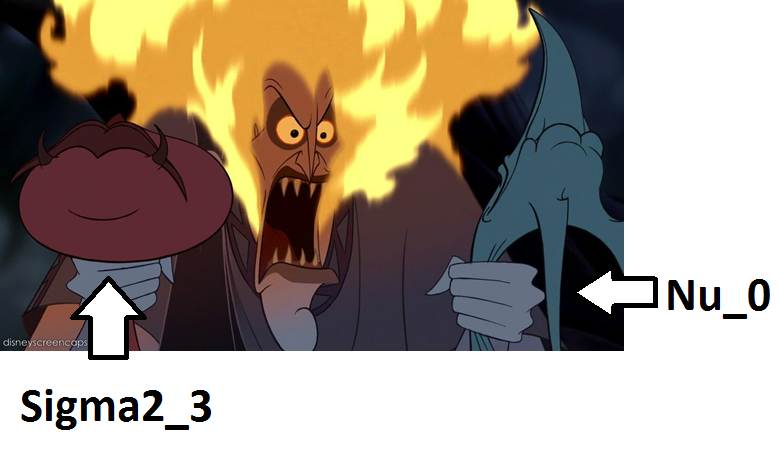
\includegraphics[width=0.9\textwidth]{hades_mad}
\end{figure}

\subsection{3.3 Algorithm output}

Estimates for parameter medians and their 95\% credible intervals are
shown in the following table:

\begin{center}
  \begin{tabular}{l c c c}
  \hline Parameter & Credible Lower 95\% & Median & Credible Upper 95\%  \\ \hline
    $\theta_1$ (Basmati) & 2.237 & 3.826 & 5.361 \\ 
    $\theta_2$ (Non-Basmati) & 4.713 & 6.240 & 7.868 \\
    $\theta_3$ (Beverage) & 0.394 & 4.841 & 9.097 \\
    $\theta_4$ (Cakes) & 3.108 & 5.200 & 7.355 \\
    $\theta_5$ (Cereal) & 1.827 & 4.042 & 6.122 \\ \hline
    $\sigma_1$ (Basmati) & 18.545 & 33.132 & 61.644 \\ 
    $\sigma_2$ (Non-Basmati) & 18.650 & 33.084 & 60.759 \\
    $\sigma_3$ (Beverage) & 131.361 & 489.618 & 3600.339 \\
    $\sigma_4$ (Cakes) & 27.028 & 50.380 & 100.924 \\
    $\sigma_5$ (Cereal) & 26.807 & 50.369 & 101.083 \\ \hline
    $\mu$ (Basmati) & 2.926 & 4.841 & 6.846 \\ 
    $\tau_2$ (Non-Basmati) & 0.573 & 2.448 & 16.913 \\
    $\nu_0$ (Beverage) & 1 & 1 & 1 \\
    $\sigma2_0$ (Beverage) & 0.277 & 1.060 & 2.712 \\ \hline
  \end{tabular}
\end{center}

\subsection{3.4 Sensitivity analyses}

We repeat the sensitivity analyses of section 1.4:

\begin{enumerate}
  \item Large expected $\mu$ (Prior expectation of mad levels of arsenic)
  \item Large $b$ and $\alpha$ (High variability within products)
  \item Large $\tau^2$ and $\eta_0$ (High variability between products)
\end{enumerate}

\textit{Scenario 1}:

\begin{center}
  \begin{tabular}{l c c c c}
  \hline Parameter & Credible Lower 95\% & Median & Credible Upper 95\% & Big change?  \\ \hline
    $\theta_1$ (Basmati) & 0.913 & 3.505 & 6.207 & Yes\\ 
    $\theta_2$ (Non-Basmati) & 4.062 & 6.686 & 9.437 & Yes \\
    $\theta_3$ (Beverage) & -32.754 & 8.074 & 71.878 & Yes \\
    $\theta_4$ (Cakes) & 1.528 & 5.485 & 9.821 & Yes \\
    $\theta_5$ (Cereal) & -0.448 & 3.504 & 7.611 & Yes \\ \hline
    $\sigma_1$ (Basmati) & 24.947 & 58.269 & 404.571 & Yes \\ 
    $\sigma_2$ (Non-Basmati) & 25.104 & 57.722 & 404.574 & Yes  \\
    $\sigma_3$ (Beverage) & 194.759 & 931.623 & 12209.972 & Yes  \\
    $\sigma_4$ (Cakes) & 36.606 & 89.011 & 626.494 & Yes  \\
    $\sigma_5$ (Cereal) & 35.694 & 89.044 & 628.468 & Yes  \\ \hline
    $\mu$ (Basmati) & 95.120  & 99.723 & 104.288 & Yes  \\ 
    $\tau_2$ (Non-Basmati) & 3033.227 & 8299.341 & 38038.052 & Yes!!  \\
    $\nu_0$ (Beverage) & 1 & 1 & 1 & No \\
    $\sigma2_0$ (Beverage) & 0.277 & 1.060 & 2.712  & Yes \\ \hline
  \end{tabular}
\end{center}

\textit{Scenario 2}:

\begin{center}
  \begin{tabular}{l c c c c}
  \hline Parameter & Credible Lower 95\% & Median & Credible Upper 95\% & Big change? \\ \hline
    $\theta_1$ (Basmati) & 1.408 & 3.479 & 5.583 & Meh\\ 
    $\theta_2$ (Non-Basmati) & 4.618 & 6.665 & 8.690 & Meh\\
    $\theta_3$ (Beverage) & -19.383 & 4.385 & 27.663 & Meh\\
    $\theta_4$ (Cakes) & 2.331 & 5.453 & 8.664 & Meh \\
    $\theta_5$ (Cereal) & 0.273 & 3.465 & 6.660 & Yes\\ \hline
    $\sigma_1$ (Basmati) & 23.249 & 47.513 & 107.471 & Meh \\ 
    $\sigma_2$ (Non-Basmati) & 23.565 & 47.531 & 106.423 & Meh \\
    $\sigma_3$ (Beverage) &  173.775 & 706.454 & 5455.201 & Meh \\
    $\sigma_4$ (Cakes) & 34.267 & 72.325 & 173.977 & Meh \\
    $\sigma_5$ (Cereal) & 33.941 & 72.486 & 174.818 & Meh \\ \hline
    $\mu$ (Basmati) & 0.456 & 4.872 & 9.262 & Yes \\ 
    $\tau_2$ (Non-Basmati) & 222.934 & 288.999 & 384.448 & Yes!! \\
    $\nu_0$ (Beverage) & 1 & 1 & 1 & No\\
    $\sigma2_0$ (Beverage) & 0.279 & 1.058 & 2.712 & Yes\\ \hline
  \end{tabular}
\end{center}

\textit{Scenario 3}:

\begin{center}
  \begin{tabular}{l c c c c}
  \hline Parameter & Credible Lower 95\% & Median & Credible Upper 95\% & Big change? \\ \hline
    $\theta_1$ (Basmati) & 1.408 & 3.479 & 5.583 & No\\ 
    $\theta_2$ (Non-Basmati) & 4.674 & 6.234 & 7.817 & No\\
    $\theta_3$ (Beverage) & 0.490 & 4.814 & 9.144 & No\\
    $\theta_4$ (Cakes) & 3.126 & 5.194 & 7.311 & No \\
    $\theta_5$ (Cereal) & 1.864 & 4.039 & 6.094 & No\\ \hline
    $\sigma_1$ (Basmati) & 18.609 & 33.008 & 60.612 & No \\ 
    $\sigma_2$ (Non-Basmati) & 18.807 & 33.083 & 61.010 & No \\
    $\sigma_3$ (Beverage) &  131.637 & 487.250 & 3367.378 & No \\
    $\sigma_4$ (Cakes) & 26.960 & 50.231 & 98.334 & No \\
    $\sigma_5$ (Cereal) & 26.904 & 50.614 & 100.647 & No \\ \hline
    $\mu$ (Basmati) & 2.926 & 4.828 & 6.741 & No \\ 
    $\tau_2$ (Non-Basmati) & 0.584 & 2.448 & 16.443 & No \\
    $\nu_0$ (Beverage) & 1 & 1 & 1 & No\\
    $\sigma2_0$ (Beverage) & 0.121 & 0.163 & 0.214 & Yes\\ \hline
  \end{tabular}
\end{center}

Results from these sensitivity analyses are analogous to those from
section 1.4; we observe that increasing \(\mu_0\) increases shrinking
towards \(\mu\) and the error on \(\theta\)'s; increasing \(a\) and
\(b\) increases the error on \(\theta\)'s and the estimates of
\(\sigma\)'s; increasing \(\tau^2_0\) and \(\eta_0\) enlarges the
credible interval around estimates of \(\sigma\)'s, along with,
obviously, \(\tau^2_0\) itself.

\subsection{3.5 Presentation of results}

\includegraphics{markdown_hw3_files/figure-latex/unnamed-chunk-21-1.pdf}
\section{4. Discussion of shrinkage}

Ignoring our failed attempt at the parameter-expanded model, we observed
greater shrinkage when modelling group-specific variances than when
setting them all equal, as the greater uncertainty on the models pulled
them closer to the prior population mean.

\section{5. Discussion of imputation}

Replacing data with mean by-group observations would simply drive down
the estimates on the errors around \(\theta\)'s, while reducing
shrinkage, driving \(\theta\)'s towards \(\bar{y}\). This follows from
\(\bar{y}\) remaining unchanged, but \(n_j\) increasing proportional to
the amount of imputed data.

\section{6. Model comparisons}

Again, we must ignore the parameter-expanded model from these
comparisons. Model 1 and 3 lead to similar inferences, although Model 3
has much greater uncertainty around the median estimates of
\(\theta\)'s. Both models clearly suggest that Basmati rice products
ought to receive special scrutiny when evaluating their arsenic
contents, whereas urgent attention seems less warranted with non-basmati
and ceraeal products. There lacks data to convincingly determine whether
rice beverage products stand exactly with relation to others.

\end{document}
